\chapter{Implementing the System: The Back-End}
	\label{chap:impl:backend}
	In chapter \ref{chap:design} the design of the solution was described. This description ranged from overall specifications, to more detailed model designs. In the following two chapters the implementation of a \emph{prototype}, following the design specifications from chapter \ref{chap:design}, is described.

	To achieve the best possibly experience for the reader, the description is split into two parts: The back-end and the front-end. In \emph{this} chapter, the implemenation of the prototype back-end is described.


	\section{The Language of the Back-End}
		When developing a REST back-end, there exists numerous tools for the job. Amongst others are Python, Node.JS, and PHP. While this list is \emph{by far} complete, it more or less states the most popular options for REST APIs and web applications, these days.

		\subsection{Python}
			One of the more popular languages for self-hosted software is Python. Python requires what is called Web Server Gateway Interface \emph{(WSGI)} server, to be able to run a webservice. Common implementations of such a server, is Django and Flask. Part of the popularity of Python is most likely the ease of which it is read. The Raspberry Pi foundation \emph{specifically} states, that:
			\begin{citequote}{rpi_python}
				``Python is a wonderful and powerful programming language that's easy to use (easy to read and write).''
			\end{citequote}

		\subsection{Node.js}
			In the later years, node.js has become more and more widespread. This is partly due to how it \emph{very} effectively handles multiple requests. While ``traditional'' sequential languages -- like python -- would spawn a thread per request, node.js uses asynchronous code and is centered around non-blocking I/O. As such, while node.js strictly speaking only ever uses one thread, it can handle \emph{massive} amounts of traffic quite easily. However, this does change the programming style of node.js programs, as it uses callback methods and JavaScript promises to a large extent. Additionally, Node.js is built ontop of Google's V8 engine, and supports C++ plugins, should it be necessary.

			One of the development advantages to node.js, is that it uses Javascript. Most web applications these days use JavaScript, and being able to code the front-end and back-end in the same language, might very well make it easier for a developer to quickly move between front-end and back-end.

		\subsection{PHP}
			PHP is without a doubt the most widespread language used for server-side scripting, when it comes to websites. However, this language can also be used to actually develop a REST api. While previously PHP would have to be executed on top of an Apache or nginx server, in newer versions PHP support a native web-server. While this, strictly speaking, is only intended for development purposes, there is nothing stopping you from running a small-scale service using this server.

		\subsection{Making A Choice}
			Taking the various options into consideration, it is concluded that the back-end will be developed using Node.js. This choice is greatly influenced by the fact that it would share development language with the front-end, thus making venturing into new territory slightly less daunting.

	\section{To Framework or Not To Framework}
		Having decided to go with Node.js for the back-end, the next big question arises: To framework or not to framework? Node.js has its own built-in webserver, and it is perfectly viable to simply use this. However, using frameworks will inevitably make it \emph{easier} to code. As such, it is decided that a framework will be used, to aid the development of the back-end.

		When it comes to these frameworks, there is no doubt that Express is the ``biggest'' one: It is simply the most widespread and popular of the frameworks available. However, alternatives such as Restify, Hapi, and Koa also exist. While these four by no means constitute the entire list of frameworks, they are the four most widely used.

		Since it has been determined in section \ref{sec:design:choosing-rest}, on page \pageref{sec:design:choosing-rest}, that the back-end essentially will be nothing more than a REST api, restify simply seems more fitting. The other frameworks contain a lot of features -- like server side rendered templates -- which simply won't be necessary when developing an API. 

		Additionally, it is noted that Restify supports limiting the SSL/TLS version, \emph{and} the available cipher-suites, as described in \ref{sec:design:secure-comms} on page \pageref{sec:design:secure-comms}. Restify supports this, using Node.js's internal HTTPS options. As such, restricting the protocol version to $TLS1.2$ is easily done using the option shown on listing \ref{lst:impl:restrict:tls1.2} on page \pageref{lst:impl:restrict:tls1.2}. Likewise, the ciphersuites being used, can be restricted using the configuration found on listing \ref{lst:impl:restrict:ciphers} on page \pageref{lst:impl:restrict:ciphers}.

		\begin{lstlisting}[style=json2,gobble=12, caption={Restricting Restify to use TLS 1.2},label={lst:impl:restrict:tls1.2}]
            secureProtocol: 'TLSv1_2_method'
		\end{lstlisting}

		\begin{lstlisting}[style=json2,gobble=12, caption={Restricting the TLS cipher suites that Restify uses. Ciphers here are \emph{examples}, as the actual list would take up too much place.},label={lst:impl:restrict:ciphers}]
            ciphers: [
                "Suite1",
                "Suite2",
                "NOT Suite3",
            ].join(':'),
            honorCipherOrder: true
		\end{lstlisting}


	\section{Node.js Coding Style}
		\label{sec:impl:node:style}
		When developing using node.js there are two different schools of thought: Callbacks and promises. Since node.js asynchronous, traditional synchronous methods should not be used. For reference purposes, the \emph{wrong} way to do it, is shown on listing \ref{lst:node:wrong} on page \pageref{lst:node:wrong}. This causes major performance issues, as the execution of the program would block, while the action taking a long time is performed.

		On listing \ref{lst:node:callback} on page \pageref{lst:node:callback}, the same output is shown using callbacks. When the data that takes a long time to produce \emph{(or fetch)} is ready, the callback is invoked, with the result. As such, while the I/O is happening the main node.js thread can continue working.

		Finally, there is listing \ref{lst:node:promise} on page \pageref{lst:node:callback}. This example uses promises, to achieve the same thing. By many, promises are thought to be the successor of callbacks. Some of the internals of the promise based method have been omitted, such as the proper use of deferreds, as this is beyond the point of this section.

		Conceptually promises are by \emph{far} the harder of the two to understand. Using them properly, without creating unnecessary overhead takes some getting used to. \emph{However} they do produce code which is \emph{much} easier to read. This is in partial due to what is commonly called ``promise chaining''. Essentially, this takes the output from one promise, and pipes it to the input for another function. 

		The above is best described using an example. In this scenario, there are three methods: \verb=fetch=, \verb=compute=, and \verb=send=, which are to be executed in that order. \verb=fetch= fetches the data from a remote source, \verb=compute= does some computations on said data, and finally \verb=send= sends the result of said computations somewhere else. On listing \ref{lst:node:callbackhell} on page \pageref{lst:node:callbackhell} this sequence of events are shown, using callbacks. As seen, the cascade of callbacks make this code \emph{horrible} to read. Professionals often use the derogatory term ``callback hell'', to describe this phenomenon. On listing \ref{lst:node:promisegoodness} on page \pageref{lst:node:promisegoodness} this \emph{exact} same sequence of events is shown, only using promises. As it is seen, this code is \emph{much} easier to read and understand. As such, using promises for this solution is by far preferable and is the style that will be used, whenever possible.

		\begin{lstlisting}[language=Javascript,gobble=12,caption={The wrong way to do it, in Node.js},label={lst:node:wrong}]
            function longTime(){
                // Something that takes a loooong time
                var res = ...
                return res;
            }
            console.log(longTime());
		\end{lstlisting}
		
		\begin{lstlisting}[language=Javascript,gobble=12,caption={Using callbacks, in Node.js},label={lst:node:callback}]
            function longTime(callback){
                // Something that takes a loooong time
                var res = ...
                callback(res);
            }
            
            longTime(function(r){
                console.log(r);
            });
		\end{lstlisting}

		\begin{lstlisting}[language=Javascript,gobble=12,caption={Using promises, in Node.js},label={lst:node:promise}]
            function longTime(){
                var deferred = Promise.defer();
                // Something that takes a loooong time
                var res = ...
                return deferred;
            }
            
            longTime()
            .then(function(r){
                console.log(r);
            })
		\end{lstlisting}

		\begin{lstlisting}[language=Javascript,gobble=12,caption={Chaining data between callbacks in node.js},label={lst:node:callbackhell}]
            get(function(data){
                compute(data, function(output){
                    send(output, function(){
                        console.log("Done!");
                    })
                })
            })
		\end{lstlisting}
		
		\begin{lstlisting}[language=Javascript,gobble=12,caption={Chaining data between promises in node.js},label={lst:node:promisegoodness}]
            get()
            .then(compute)
            .then(send)
            .then(function(){
                console.log("Done!");
            })
		\end{lstlisting}

	\section{Structuring the Codebase}
		\label{sec:impl:backend:codebase}
		When it comes to a codebase's readability and maintainability, a good structure is almost the most important thing. As such, a proper categorisation is the first thing needed. Fundamentally, there will be four different types of code files, in the project: Models, routes, tests, and middleware.

		Models represent on-disk data structures, as will be stored in the database. These were covered in section \ref{sec:modelling} on page \pageref{sec:modelling}. Since node.js natively supports ECMAScript 6 objects, these models will be represented as objects in memory. The models also contains the relevant methods for manipulating the entries. An example of this could be looking up a user, from an ID.

		Routes represent API endpoints. These are described in full detail, in section \ref{sec:impl:api} on page \pageref{sec:impl:api}. These routes will be separated into files representing their primary resource.

		Tests should hopefully be obvious. These are the unittests for the back-end. Further details regarding testing framework and methodology is found in section \ref{sec:impl:tests} on page \pageref{sec:impl:tests}.

		Middleware would be the last category. What exactly these are, is explained in further details in section \ref{sec:impl:middleware} on page \pageref{sec:impl:middleware}.

		As such, the basic structure of the back-ends codebase will be as follows:
		\dirtree{%
		.1 project.
		.2 app.js.
		.2 middlewares.
		.2 models.
		.2 routes.
		.2 tests.
		}

	\section{Database Abstraction Layer}
		As decided in section \ref{sec:restrict:database} on page \pageref{sec:restrict:database}, a database abstraction layer is necessary. While Object-Relational Mapping \emph{(ORM)} strictly speaking isn't the same as a DAL, for this section the two are considered equivalent.

		The three most widely used solutions for this, is Sequelize, Bookshelf, and Knex \emph{(Bookshelf is built ontop of Knex)}. Sequelize and Bookshelf are both ORMs, whereas Knex is a DAL. In regards to platform support, they are fairly similar. Sequelize supports PostgreSQL, MySQL, SQLite and MSSQL. Bookshelf/Knex supports MySQL, SQLite, Postgres, MariaDB, and Oracle.

		While working with ORMs generally takes database interactions to a higher abstraction level, it is found that the ease of which Knex's query builder work, makes it a lot easier to just write these queries directly. Additionally, Knex allows for querying using Promises, which ensures that it will integrate nicely with the style argued for in section \ref{sec:impl:node:style} on page \pageref{sec:impl:node:style}. As such, it is concluded the Knex is the superior choice as a DAL for the implementation.

	\section{API Endpoints}
		\label{sec:impl:api}
		Before defining the endpoints, the resources \emph{(see section \ref{sec:design:rest} on page \pageref{sec:design:rest})} of the application need to be determined. Looking at the models defined in section \ref{sec:modelling} on page \pageref{sec:modelling}, these offer a great starting point for identifying resources.

		\subsection{The Users Resource}
			First and foremost there is the collection of Users. This collections represents the user base as a whole. \verb=POST=ing to this collection would -- by extension -- mean the creation of a new user. \verb=GET=ing the user collection, mean retrieving all user entries, with their username and other attributes in the ``public domain''. \verb=PUT= and \verb=DELETE= is slightly different. They're used for updating and deleting a \emph{single} user, in the entire collection. As such, the endpoint needs to have a user ID postfixed. Adhering to the standard, \emph{all} API endpoints will have \verb=/api= prefixed. These API endpoints are listed on table \ref{tab:api:users} on page \pageref{tab:api:users}.

		\subsection{The Passwords Resource}
			Then there is the collection of passwords. However, there is a slight caveat when it comes to this collection. Since each password is \emph{owned} by a user, it can thought be thought that there exists \emph{multiple} collections -- one for each user. As such, the password collection is stored behind the user resource and the ID specifying exactly which user owns said password. The same approach to designing these endpoints are used, as with the user resource and the result of this is found on table \ref{tab:api:passwords} on page \pageref{tab:api:passwords}.

			For simplicity's sake, access to shared passwords is stored behind the passwords resource. As such, a collection called shares -- which belongs to a specific password -- denotes the collection of users this specific password has been shared to. Additionally, two collections are added as well: \verb=shared= and \verb=shares=. These two are  \emph{very} similar in name, which unfortunately might result in some confusion. The \verb=shares= resource denotes passwords shared \emph{to} the user and the \verb=shared= resource denotes passwords that the user has shared to \emph{others}. These endpoints are found on table \ref{tab:api:sharedpasswords} on page \pageref{tab:api:sharedpasswords}.

		\subsection{The Categories Resource}
			The same argument made in regards to the passwords collection, can be said about categories. Each user has their own private password collection, which is -- similar to passwords -- stored behind the owning user's ID. This can be seen on table \ref{tab:api:categories} on page \pageref{tab:api:categories}.

		\subsection{The Invites Resource}
			When an admin creates a new invites, it can be said he \verb=POST=s it to the invites resource. \verb=GET=ing an ID, returns the status of an ID stored in the database. Then, there is finally the act of using an invite. Since a user is created, it only makes sense that the \verb=POST= method is needed. However, since the regular endpoint is already being posted to, an additional endpoint is needed. As such, appending the endpoint with \verb=/accept= will achieve this. This can be seen on table \ref{tab:api:invites} on page \pageref{tab:api:invites}.

		\subsection{The Audit Resource}
			The Audit resource is extremely simple. It only consists of a single endpoint: Reading the audit log. Since this resource is owned by individual users, this is -- much like passwords and categories -- stored behind the user collection and a specific ID. This can be seen on table \ref{tab:api:audit} on page \pageref{tab:api:audit}.

		\subsection{The Auth Resource}
			\label{sec:api:auth}
			The Auth resource is a little bit more interesting. Of course, there is the generic \verb=POST=, containing the user's username and password, for authentication purposes. The details of this is covered in section \ref{sec:design:authentication} on page \pageref{sec:design:authentication}. However, this is not all. Since the solution supports TOTP two-factor-authentication, as described in section \ref{sec:mfa} on page \pageref{sec:mfa}, endpoints for enabling this is needed as well. 

			In section \ref{sec:design:breaking-rest} on page \pageref{sec:design:breaking-rest} it was argued that at one point it would be \emph{necessary} to break the REST principles. This is when. As such, two endpoints are needed: One for generating a new secret and caching it, and one for actually verifying said secret.


		
		\newcolumntype{L}[1]{>{\hsize=#1\hsize\raggedright\arraybackslash}X}%
		\newcolumntype{R}[1]{>{\hsize=#1\hsize\raggedleft\arraybackslash}X}%
		\newcolumntype{C}[2]{>{\hsize=#1\hsize\columncolor{#2}\centering\arraybackslash}X}%
		
		\begin{table}[p]
			\definecolor{tablerow1}{RGB}{230,230,230}
			\definecolor{tablerow2}{RGB}{255,255,255}
			\rowcolors{2}{tablerow1}{tablerow2}
			
			\begin{tabularx}{\textwidth}{ R{0.15} | L{0.65} | L{0.2} }
				\bfseries Method & \bfseries Endpoint & \bfseries Description% specify table head
				\csvreader[head to column names]{resources/api/users.csv}{}% use head of csv as column names
				{\\\hline\method & \texttt{\endpoint} & \description}% specify your coloumns here
			\end{tabularx}

			\caption{API endpoints for the Users resource.}
			\label{tab:api:users}
		\end{table}


		\begin{table}[p]
			\definecolor{tablerow1}{RGB}{230,230,230}
			\definecolor{tablerow2}{RGB}{255,255,255}
			\rowcolors{2}{tablerow1}{tablerow2}
			
			\begin{tabularx}{\textwidth}{ R{0.15} | L{0.65} | L{0.2} }
				\bfseries Method & \bfseries Endpoint & \bfseries Description% specify table head
				\csvreader[head to column names]{resources/api/passwords.csv}{}% use head of csv as column names
				{\\\hline\method & \texttt{\endpoint} & \description}% specify your coloumns here
			\end{tabularx}

			\caption{API endpoints for the Passwords resource.}
			\label{tab:api:passwords}
		\end{table}

		\begin{table}[p]
			\definecolor{tablerow1}{RGB}{230,230,230}
			\definecolor{tablerow2}{RGB}{255,255,255}
			\rowcolors{2}{tablerow1}{tablerow2}
			
			\begin{tabularx}{\textwidth}{ R{0.15} | L{0.65} | L{0.2} }
				\bfseries Method & \bfseries Endpoint & \bfseries Description% specify table head
				\csvreader[head to column names]{resources/api/sharedPasswords.csv}{}% use head of csv as column names
				{\\\hline\method & \texttt{\endpoint} & \description}% specify your coloumns here
			\end{tabularx}

			\caption{API endpoints for accessing Shared Passwords.}
			\label{tab:api:sharedpasswords}
		\end{table}		

		\begin{table}[p]
			\definecolor{tablerow1}{RGB}{230,230,230}
			\definecolor{tablerow2}{RGB}{255,255,255}
			\rowcolors{2}{tablerow1}{tablerow2}
			
			\begin{tabularx}{\textwidth}{ R{0.15} | L{0.65} | L{0.2} }
				\bfseries Method & \bfseries Endpoint & \bfseries Description% specify table head
				\csvreader[head to column names]{resources/api/categories.csv}{}% use head of csv as column names
				{\\\hline\method & \texttt{\endpoint} & \description}% specify your coloumns here
			\end{tabularx}

			\caption{API endpoints for the Categories resource.}
			\label{tab:api:categories}
		\end{table}
		
		\begin{table}[p]
			\definecolor{tablerow1}{RGB}{230,230,230}
			\definecolor{tablerow2}{RGB}{255,255,255}
			\rowcolors{2}{tablerow1}{tablerow2}
			
			\begin{tabularx}{\textwidth}{ R{0.15} | L{0.65} | L{0.2} }
				\bfseries Method & \bfseries Endpoint & \bfseries Description% specify table head
				\csvreader[head to column names]{resources/api/invites.csv}{}% use head of csv as column names
				{\\\hline\method & \texttt{\endpoint} & \description}% specify your coloumns here
			\end{tabularx}

			\caption{API endpoints for the Invites resource.}
			\label{tab:api:invites}
		\end{table}

		\begin{table}[p]
			\definecolor{tablerow1}{RGB}{230,230,230}
			\definecolor{tablerow2}{RGB}{255,255,255}
			\rowcolors{2}{tablerow1}{tablerow2}
			
			\begin{tabularx}{\textwidth}{ R{0.15} | L{0.65} | L{0.2} }
				\bfseries Method & \bfseries Endpoint & \bfseries Description% specify table head
				\csvreader[head to column names]{resources/api/audit.csv}{}% use head of csv as column names
				{\\\hline\method & \texttt{\endpoint} & \description}% specify your coloumns here
			\end{tabularx}

			\caption{API endpoint for the Audit resource.}
			\label{tab:api:audit}
		\end{table}

		\begin{table}[p]
			\definecolor{tablerow1}{RGB}{230,230,230}
			\definecolor{tablerow2}{RGB}{255,255,255}
			\rowcolors{2}{tablerow1}{tablerow2}
			
			\begin{tabularx}{\textwidth}{ R{0.15} | L{0.65} | L{0.2} }
				\bfseries Method & \bfseries Endpoint & \bfseries Description% specify table head
				\csvreader[head to column names]{resources/api/auth.csv}{}% use head of csv as column names
				{\\\hline\method & \texttt{\endpoint} & \description}% specify your coloumns here
			\end{tabularx}

			\caption{API endpoints for the Auth resource.}
			\label{tab:api:auth}
		\end{table}

	\section{Workaround To Be Self-Contained}
		\label{sec:impl:backend:restify-fix}
		Unfortunatly, Restify's documentation is at some points less than ideal. They have what they call the serveStatic method. From their description, its intended use is to deliver a default file, if a match is not found. This is exactly what is needed for the front-end's router \emph{(more on this in section \ref{sec:impl:ui-router} on page \pageref{sec:impl:ui-router})}. However, after much fiddling, it was found simply not to work.

		As such, a workaround is needed. After having defined \emph{all} of the API routes, six new routes are defined as is seen on table \ref{tab:api:workaround} on page \pageref{tab:api:workaround}. This ensures that any API hits are given the proper error code, while ensuring that the application for the front-end is being delivered in all cases.
		
		\begin{table}[p]
			\definecolor{tablerow1}{RGB}{230,230,230}
			\definecolor{tablerow2}{RGB}{255,255,255}
			\rowcolors{2}{tablerow1}{tablerow2}
			
			\begin{tabularx}{\textwidth}{ R{0.15} | L{0.65} | L{0.2} }
				\bfseries Method & \bfseries Endpoint & \bfseries Description\\% specify table head
				GET 	& 	/api/.* 	& Returns error 404 Not Found \\
				HEAD 	& 	/api/.* 	& Returns error 404 Not Found \\
				POST 	& 	/api/.* 	& Returns error 404 Not Found \\
				PUT 	& 	/api/.* 	& Returns error 404 Not Found \\
				DEL 	& 	/api/.* 	& Returns error 404 Not Found \\
				PATCH 	& 	/api/.* 	& Returns error 404 Not Found \\
			\end{tabularx}

			\caption{Workaround error routes, to make the API adhere to standards and the front-end's router to work \emph{(see section \ref{sec:impl:ui-router} on page \pageref{sec:impl:ui-router})}.}
			\label{tab:api:workaround}
		\end{table}


%		\begin{table}
%			\centering
%			\begin{tabular}{r | l}
%				\textbf{Method} & \textbf{Endpoint} \\
%				\hline
%				\verb=GET=		& \verb=/api/.*= \\
%				\verb=HEAD=		& \verb=/api/.*= \\	
%				\verb=POST=		& \verb=/api/.*= \\	
%				\verb=PUT=		& \verb=/api/.*= \\
%				\verb=DEL=		& \verb=/api/.*= \\
%				\verb=PATCH=	& \verb=/api/.*= \\	
%			\end{tabular}
%			\caption{Workaround error routes, to make the API adhere to standards and the front-end's router to work \emph{(see %section \ref{sec:impl:ui-router} on page \pageref{sec:impl:ui-router})}}%
%			\label{tab:api:workaround}%
%		\end{table}
%
	\section{Validating Input}
		Whenever a system is developed, that requires the input of a user, it is generally a bad idea to blindly trust that the input is \emph{correct}. As such, validating the input JSON is necessary. There exists a plethora of tools for this \emph{exact} purpose. 

		Unfortunately, this is the place where the nature of humans comes into play. When development of the solution started, the tool schemagic was selected. At the time, it seemed the simplest of the available libraries. However, last few weeks of the project, the library ajv began to seem more and more appropriate, albeit a bit more difficult to setup. Unfortunately, it was deemed necessary to \emph{not} migrate to the new tool, due to a lack of time. However, this is \emph{definitely} something that will need to be done in the future.

		\subsection{Using ajv}
			Using ajv is as simple as defining a scheme. This scheme defines the allowed variables that the input json can, may, or should contain. On listing \ref{lst:json:ajv:password} on page \pageref{lst:json:ajv:password} an example of this is found. It stated that a password entry \emph{must} contain a title \emph{(string)} and a password \emph{(base64 encoded string)}, and \emph{can} contain a username, url, note, and a parent \emph{(parent field defaults to null)}. The \verb=user.schema= variable can then be used as a \emph{promise} to verify input. This is seen on listing \ref{lst:json:ajv:password:use} on page \pageref{lst:json:ajv:password}. The fact that ajv supports validation using promises, is a huge advantage, in regards to readability, as per section \ref{sec:impl:node:style} on page \pageref{sec:impl:node:style}.

			\begin{lstlisting}[gobble=16,language=JavaScript,caption={JSON schema for the password model, using ajv's notaiton.},label={lst:json:ajv:password},breakatwhitespace=false]
                var schema = {
                    "$async": true,
                    "properties": {
                        "title": {
                            "type": "string"
                        },
                        "username": {
                            "type": "string"
                        },
                        "password": {
                            "type": "string",
                            "pattern": "^([A-Za-z0-9+\/]{4})*([A-Za-z0-9+\/]{4}|[A-Za-z0-9+\/]{3}=|[A-Za-z0-9+\/]{2}==)$"
                        },
                        "parent": {
                            "type": "number"
                        },
                        "url": {
                            "type": "string"
                        },
                        "note": {
                            "type": "string"
                        }
                    },
                    "required": [ "title", "password" ],
                    "additionalProperties": false
                };
                var user = {
                    schema = ajv.compile(schema);
                }
				\end{lstlisting}

			\begin{lstlisting}[gobble=16,language=JavaScript,caption={Using the user schema for validating input, using ajv.},label={lst:json:ajv:password:use}]
                validate({title: 'I Love Programming', 'password': 'V2hhdC4uLiBBZ2Fpbj8h'))
                .then(function (valid) {
                    console.log('Data is valid');
                })
                .catch(function (err) {
                    console.error('Validation errors:', err.errors);
                });
		\end{lstlisting}

	\section{Authentication}
		\label{sec:impl:authentication}
		In section \ref{sec:api:auth} on page \pageref{sec:api:auth} the endpoints involved in authentication was described. In this section, the process is described a little further. 

		As with any authentication, the user starts by sending his or her username and password \emph{(see section \ref{sec:design:authentication} on page \pageref{sec:design:authentication})}. If two factor authentication is not enabled, the standard verification approach is made. If the password matches, http code \verb=200= is returned, signifying successful authentication. Should it not match, http code \verb=401= is returned, signifying unsuccessful authentication.

		Should two factor authentication be enabled, however, a more complex event happens. Since the front-end won't know if two factor authentication is enabled or not, this needs to be conveyed to it. As such, should the user have two-factor authentication enabled, but the token is missing from the body, http error code \verb=403= is returned. \verb=403= is defined as follows, by RFC2616\cite{httpcodes}:
		\begin{citequote}[sec.10.4.4]{httpcodes}
				``The server understood the request, but is refusing to fulfill it...''
		\end{citequote}
		When the front-end receives the \verb=403= from the authentication endpoint, it \emph{knows} to promt to the user for a two-factor-token. Once this token is obtained, the request is sent again -- with the token. Once received, the back-end verifies the password, similar to before, and verifies that the token is correct. If all fields are verified the back-end responds with \verb=200= to signify successful authentication. Should either field fail to be verified, the response is \verb=401= to signify unsuccessful authentication. Figure \ref{fig:sequence:auth} on page \pageref{fig:sequence:auth} depicts this series of event, in a sequence diagram.

		Upon successful authentication -- either with or without 2FA -- a JWT will be issued, in accordance with section \ref{sec:design:jwt} on page \pageref{sec:design:jwt}. This token is signed, using the back-ends private-key specifically intended for this use. For future reference, this key is known as the private-JWT-key.

		\begin{figure}[p]
			\centering
			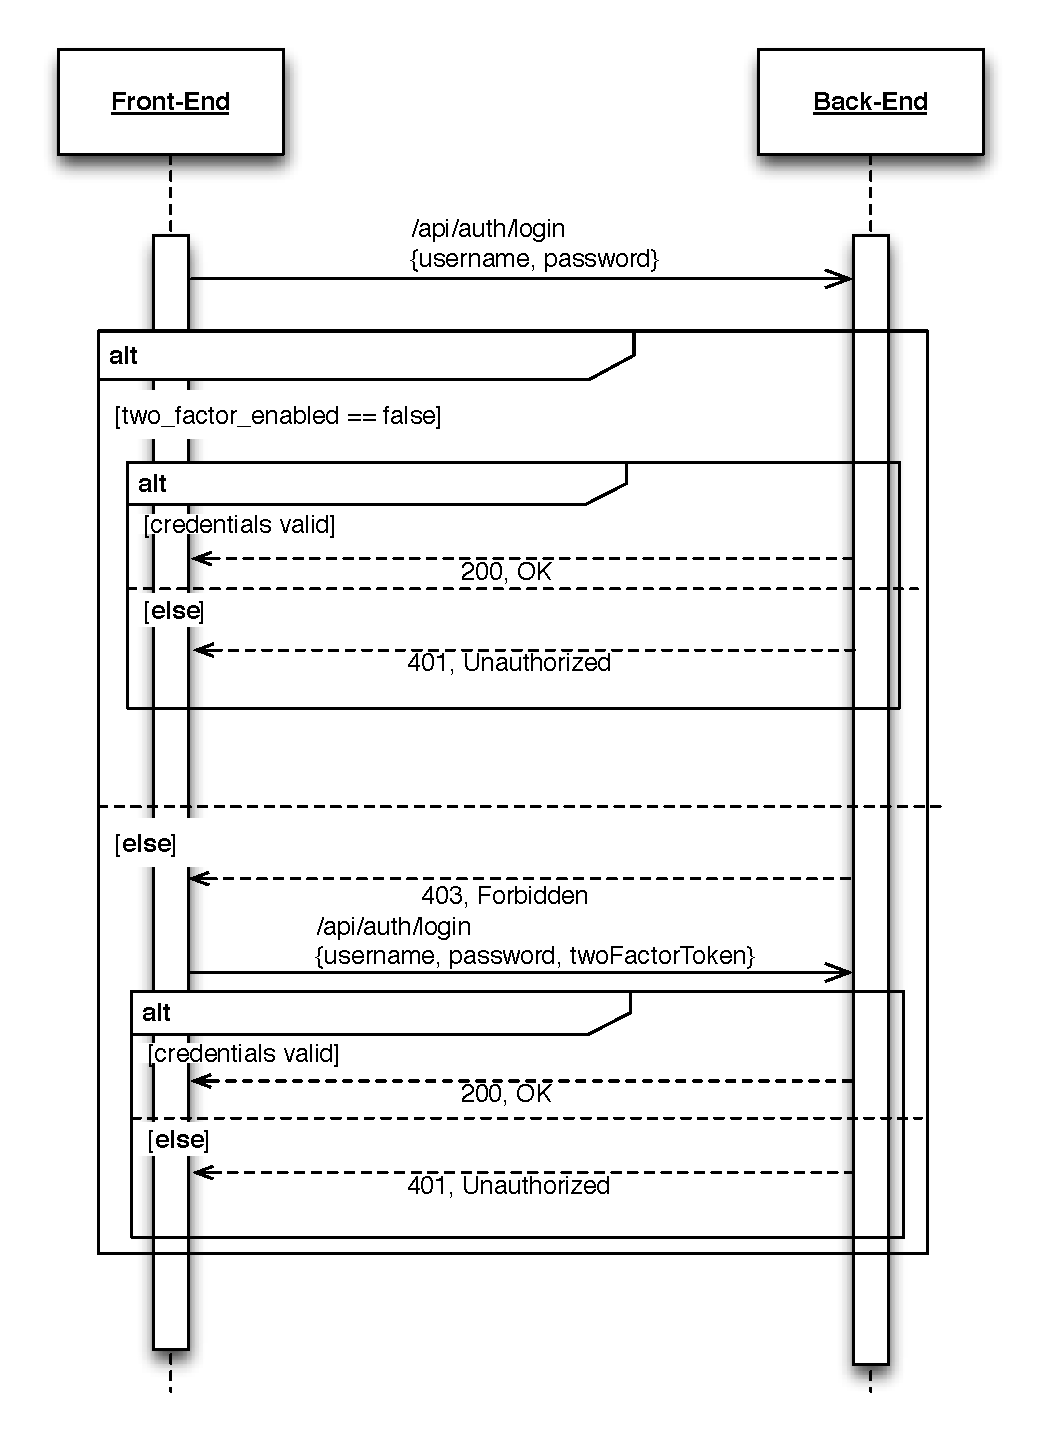
\includegraphics[width=0.8\textwidth]{figures/implementation/uml/sequence/authentication.eps}
			\caption{Sequence diagram showing the process of how the front-end authenticates to the back-end.}
			\label{fig:sequence:auth}
		\end{figure}

		%\subsection{Deviating from the Design}
			%Unfortunately, it is necessary to deviate from the design here. Where section \ref{sec:password} on page \pageref{sec:password} dictated that the Argon2 algorithm should be used for password hashing, it is simply not feasible. There currently only exist one binding for this, for node.js, and unfortunately using this binding, results in an inability to run it on ARM platforms.

			%As such, it is necessary to simply use a tried and tested algorithm, namely PBKDF2. This is also mentioned in OWASP's recommendations\cite{owasp_kdf}.

		\subsection{Powering the Two-Factor Authentication}
			To aid in the development, a third party tool is chosen for aiding the two-factor authentication. The Speakeasy project\cite{speakeasy_lib} is not only well documented and extremely easy to use, it is also pretty much the only two-factor authentication tool for Node.js, that has any credibility at all. As such, the choice fell on this suite.

			Speakeasy not only makes appropriate TOTP secret generation easy, but also makes verifying a token extremely easy. The snippet for verification is found on listing \ref{lst:example:speakeasy:verification} on page \pageref{lst:example:speakeasy:verification} \emph{(example taken from their GitHub repository)}. \verb=base32secret= is the secret that the TOTP client and the back-end has in common, and \verb=userToken= is the TOTP token.


			\begin{lstlisting}[gobble=16,language=JavaScript,caption={Verifying a TOTP token using Speakeasy},label={lst:example:speakeasy:verification}]
                var verified = speakeasy.totp.verify({ secret: base32secret, encoding: 'base32', token: userToken });
			\end{lstlisting}
	
	\section{Middlewares}
		\label{sec:impl:middleware}
		To ease implementation and to reduce code duplication, certain features will be implemented using what is commonly known as middlewares. Middlewares are simply a term for methods, being executed \emph{before} the actual controller of an endpoint. An example of an endpoint is:
		\begin{lstlisting}[gobble=12,language=JavaScript]
            server.get('/api/ping', function(req, res, next){
                res.send(200, 'OK');
                return next();
            });		
		\end{lstlisting}

		Whenever \emph{any} client performs a HTTP call to the endpoint \verb=/api/ping=, using the \verb=GET= method, the server simply returns http code \verb=200=, and continues its operation. However, a new middleware will now be created. This middleware will effectively \emph{log} whenever a ping request is made. The code for the logger is found on listing \ref{lst:example:pinglog} on page \pageref{lst:example:pinglog}. Listing \ref{lst:example:ping_wlog} on page \pageref{lst:example:ping_wlog} now contains the updated ping endpoint. As is seen on line 2, the variable \verb=pinglog= is injected into the route handler. As such, the code on listing \ref{lst:example:pinglog} is executed \emph{before} the code from listing \ref{lst:example:ping_wlog}, \emph{every} single time.

		\begin{lstlisting}[gobble=12,language=JavaScript,caption={PingLog Middleware},label={lst:example:pinglog}]
            module.exposts = function(req, res, next){
                console.log('Ping reqeuest received');
                return next();
            }
		\end{lstlisting}

		\begin{lstlisting}[gobble=12,language=JavaScript,caption={Ping endpoint with the pinglog middleware},numbers=left,label={lst:example:ping_wlog}]
            var pinglog = require('pinglog.js');
            server.get('/api/ping', pinglog, function(req, res, next){
                res.send(200, 'OK');
                return next();
            });		
		\end{lstlisting}

		This design approach is used for several features in the codebase, most noticeable:
		\begin{itemize}
			\item Object Resolving \emph{(see section \ref{sec:impl:resolve} on page \pageref{sec:impl:resolve})}
			\item Token Verification \emph{(see section \ref{sec:impl:token-verification} on page \pageref{sec:impl:token-verification})}
			\item Authorization \emph{(see section \ref{sec:impl:authorization} on page \pageref{sec:impl:authorization})}
		\end{itemize}

	\section{Token Verification}
		\label{sec:impl:token-verification}
		In section \ref{sec:impl:authentication} on page \pageref{sec:impl:authentication} it was discussed how the JWTs are issued, \emph{(see section\ref{sec:design:jwt} on page \pageref{sec:design:jwt})}. Since most endpoints will require an authenticated user, this makes token verification a \emph{prime} candidate for implementation as a middleware.

		Verifying these tokens are \emph{extremely} simple. When issued, they're signed with the server's private-JWT-key, \emph{(see section \ref{sec:impl:authentication} on page \pageref{sec:impl:authentication})}. Verification is simply making sure, that the received token \emph{was} signed with the back-ends own private-JWT-key.

		Upon successful token verification, the corresponding user object is fetched from the database, and attached to the request, as the \verb=req.resolved.user= variable, which subsequent middlewares and controllers can access. 

	\section{Resolving Objects}
		\label{sec:impl:resolve}
		Since multiple routes exists for the same type of objects \emph{(get, post, put and delete)}, it would be beneficial to have a single place, where objects are read from the database. As such, a common object resolving middleware is made. It requires a number of standards, however. First and foremost, all object IDs found in the URL is to be postfixed with a constant, \verb=Id=. This is done to easily manipulate the variable name string, to identify the corresponding object. Secondly, \emph{all} resolvable objects \emph{must} use the same method definition to lookup an object from the database, using their ID: The \verb=find(..)= method.

		Using these two constraints, a resolver can fairly easily be built. It simply strips the tailing two characters from the variable name, and based on the rest it looks up a user, a password, a category, an invite, or a shared password. The core of the resolver is found on listing \ref{lst:example:resolver} on page \pageref{lst:example:resolver}. The \verb=objectTypes= array is used for creating the final variable names, which the controllers will then refer to these objects as.

		\begin{lstlisting}[gobble=12,language=JavaScript,caption={Object resolver middleware},label={lst:example:resolver}]
            _.mapObject(req.params, function(val, key){
            
                // If the name is not present in classNames array, we're
                // dealing with a body parameter and should skip.
                if( key.slice(-2) === 'Id' && classNames[key.slice(0, -2)] !== undefined ){
                    
                    // Creating empty JSON object for the resolved objects to be placed in
                    if( req.resolved.params === undefined ) 
                        req.resolved.params = {};
                    
                    objectTypes.push(key.slice(0, -2));
                    objects.push( (classNames[key.slice(0, -2)]).find(val) );
                }
            
            });
		\end{lstlisting}

		All of the resolved objects, are then attached to the request, before being passed on to the next handler. Resolved objects are found in the \verb=req.resolved.params= variable, which subsequent middlewares and controllers can access.

	\section{Authorization}
		\label{sec:impl:authorization}
		For authorization purposes two strategies will be used: Simple and advanced authorization. For all purposes where simple authorization is a possibility, it will be used. In section \ref{sec:design:authorization} on page \pageref{sec:design:authorization} it was described which users has access to which entities. The following two sections will adhere to this design.

		\subsection{Basic Authorization}
			%Using the API described in section \ref{sec:impl:api} on page \pageref{sec:impl:api}, it is clearly seen that models' IDs are found in the URL. As such, using the owner field, of these models, it can easily be determined if the authenticated user has access to any given resource.
			In the previous too sections, the token verification \emph{(section \ref{sec:impl:token-verification})} and object resolving  \emph{(section \ref{sec:impl:resolve})} middleware were explained. Using these resolved objects' IDs, a very simple authorization scheme can be devised.

			As per the design, \emph{both} the user and admins will have full access to all user methods. This is simply handled with a comparison:
			\begin{lstlisting}[gobble=16,language=JavaScript]
                if( req.resolved.user.id === user.id || req.resolved.user.isAdmin ){
			\end{lstlisting}

			Since it is only the user self, that has access to his or her passwords, this is also handled extremely easy by doing:
			\begin{lstlisting}[gobble=16,language=JavaScript]
                if( password.owner === user.id && user.id === req.resolved.user.id ){
			\end{lstlisting}
			The exact same is done for categories:
			\begin{lstlisting}[gobble=16,language=JavaScript]
                if( category.owner === user.id && user.id === req.resolved.user.id ){
			\end{lstlisting}

			Shared passwords however, are a little bit more difficult. As has already been stated, both the user \emph{sharing} the password and the user receiving the shared password needs access to this resource. As such, the logic is a little different:
			\begin{lstlisting}[gobble=16,language=JavaScript]
                if( (share.owner === user.id && user.id === req.resolved.user) || (share.origin_owner === user.id && user.id === req.resolved.user)){
			\end{lstlisting}
		
			If the above snippets are evaluated to \verb=true=, the code keeps executing. If it is evaluated to false, the back-end returns http code \verb=403=, Forbidden denoting that the user does \emph{not} have sufficient privileges to access that specific data.

		\subsection{Advanced Authorization}
			However, this only works on select resources. As the user will easily see, the invite endpoints will not work using the simple method. As such, the groundwork for a more advanced and fine grained authorization framework is made.

			First and foremost, the basic target is defined. In this case, it will be \verb=invite=. Next, the actions on this target is defined. For invites, there really only is one: \verb=create=. For other objects, these actions might be \verb=update=, \verb=delete=, etc. Then, for each target, each method's permissions can be defined. For each endpoint, the middleware is given a variable, \verb=permObject= \emph{(permissions object)}, which denotes the resource and action in question. In the invites case, the following snippet shows the authorization process:

			\begin{lstlisting}[gobble=16,language=JavaScript]
                function invite(permObject, req, res, next){
                    // Supported Methods
                    var methods = ['create'];
                    
                    // Check to see if method is supported in authorization suite
                    if( _.indexOf(methods, permObject.method) === -1 ){
                        return deny(next);
                    }
                    
                    if( permObject.method === methods[0] ){
                        // Allow creation of invite, if the user is an admin
                        if( req.resolved.user.isAdmin ){
                            return next();
                        }

                        return next(new restify.errors.ForbiddenError('Insufficient privileges'));
                    }
                }			
			\end{lstlisting}
			The \verb=deny(..)= method is just a wrapper to elegantly throw the same error, across multiple authorization targets. The content of this method is as simple as:
			\begin{lstlisting}[gobble=16,language=JavaScript]
                function deny(next){
                    return next(new restify.errors.ForbiddenError('Insufficient privileges'));
                }
			\end{lstlisting}

		\subsection{Simple or Advanced}
			There is not a seconds doubt that the advanced approach is more fine grained. Where the simple approach only supports differentiating between targets, the advanced approach also supports differentiating between actions. As such, while the simple method does its job perfectly as is, should the need for more detailed authorization options arise, they will need to be implemented the advanced approach.


	\section{Handling Errors}
		Using the Bluebird.js promise library, error handling in the back-end is simplified a lot. Whereas native promises generally only support catching \emph{all} errors, Bluebird supports filtered catching: Custom errors can be extended from the default error, creating very easy separation of error type. 

		On listing \ref{lst:example:errorhandle:password:create} on page \pageref{lst:example:errorhandle:password:create} an example snippet is shown. It shows the error catching when creating a new password. This process can throw one of three errors: \verb=UserDoesNotExistError=, \verb=ValidationError=, and \verb=SqlError=. While these are not the only errors that the back-end can throw, it is a selection. For a full list of available errors, please refer to appendix \ref{appendix:errors:backend}.

		\begin{lstlisting}[language=Javascript,gobble=12,caption={Example of error handling, when creating new password},label={lst:example:errorhandle:password:create}]
            Password.create(password)
            .then(function(password){
                // Handle the error
            })
            .catch(UserDoesNotExistError, function(err){
                // Handle the error
            })
            .catch(ValidationError, function(err){
                // Handle the error
            })
            .catch(SqlError, function(err){
                // Handle the error
            });
		\end{lstlisting}

	\section{Testing the API}
		\label{sec:impl:tests}
		Last but not least, testing of the back-end is -- of course -- necessary. One could go about manually creating the HTTP requests and testing the output, but this is far from efficient.

		As such, unittesting is necessary. One of the most popular frameworks for unittesting in the JavaScript community is without a doubt mocha. However, since this is an API that will be tested, mocha isn't \emph{enough}. When testing the HTTP calls there are two approaches: Either the actual server is run in a separate process, or the test framework runs the server itself. However, running the server separately will \emph{quickly} become very tedious, since it would have to be restarted for each set of tests. 

		Fortunately, there exists a tool designed \emph{specifically} to aid in this type of unittesting: Supertest. It simply plugs into the main application code, and bootstraps a local version of the routes themselves. Then tests can be run on this, \emph{as if} it was running in a separate process. The application code simply has to export a link to the primary object \emph{(often the server or app variable)}, whenever the \verb=process.env.NODEENV= environment variable is set to \verb=test=. This export is shown on listing \ref{lst:impl:backend:testexport} on page \pageref{lst:impl:backend:testexport}. This is then used in Supertest, in order to test the result of certain requests. This is seen on listing \ref{lst:impl:backend:supertest} on page \pageref{lst:impl:backend:supertest}. 

		As seen, when \verb=POST=ing to the endpoint \verb=/api/auth/login= \emph{(as described in section \ref{sec:impl:api} on page \pageref{sec:impl:api})}, with the username ``daniel'' and the password ``password'', it is \emph{expected} that it returns HTTP code \verb=200=, which indicates a successful authentication.


		\begin{lstlisting}[language=Javascript,gobble=12,caption={Application's export of primary variable, when in test environment},label={lst:impl:backend:testexport}]
            if( process.env.NODE_ENV === 'test' ){
                module.exports = server;
            }else{
                server.listen(opts.port);
            }
        \end{lstlisting}

		\begin{lstlisting}[language=Javascript,gobble=12,caption={Unittesting API endpoints, using Supertest},label={lst:impl:backend:supertest}]
            var request = require('supertest');  
            var server  = request(require(__base + 'app.js').server);
            
            server
            .post('/api/auth/login')
            .field('username', 'daniel')
            .field('password', 'password')
            .expect(200)
		\end{lstlisting}

		Finally, there is the question of \emph{code coverage}. Using the tool Istanbul, the coverage of the unittesting of the back-end is calculated. The result of this is found on figure \ref{lst:impl:coverage} on page \pageref{lst:impl:coverage}. While $100\%$ code coverage should be strived for, achieving $77.59\%$ is far from bad.

		\lstinputlisting[language={},caption={Code coverage results, using Istanbul. Some equality signs removed to fit on a single page.},label={lst:impl:coverage}]{resources/coverage.txt}

































